\documentclass{article}
\usepackage[utf8]{inputenc}
\usepackage{tikz}
\parindent0pt
\def\globalscale {0.01350000}


%%%%%   symbols map   %%%%%
% # 3. other symbols (31)
% OTHER_SYMBOLS = {
%     "!": "exclam",
%     '"': "quotedbl",
%     "#": "numbersign",
%     "$": "dollar",
%     "%": "percent",
%     # " ": "space", # ignore space symbol
%     "&": "ampersand",
%     "'": "quotesingle",
%     "(": "parenleft",
%     ")": "parenright",
%     "*": "asterisk",
%     "+": "plus",
%     ",": "comma",
%     "-": "hyphen",
%     ".": "period",
%     "/": "slash",
%     ":": "colon",
%     ";": "semicolon",
%     "<": "less",
%     "=": "equal",
%     ">": "greater",
%     "?": "question",
%     "@": "at",
%     "[": "bracketleft",
%     "\\": "backslash", # backslash '\'
%     "]": "bracketright",
%     "^": "asciicircum",
%     "_": "underscore",
%     "`": "grave",
%     "{": "braceleft",
%     "|": "bar",
%     "}": "braceright",
%     "~": "asciitilde",
%     }


\begin{document}
%%%%%     TEST for 'lmr' other symbols      %%%%%
\section{lmr other symbols}
% 1. '@' symbol:
XXX%

\begin{tikzpicture}[y=1cm, x=1cm, yscale=\globalscale,xscale=\globalscale, every node/.append style={scale=\globalscale}, inner sep=0pt, outer sep=0pt]
\path [draw=red, fill=teal, scale=2, line width=.15pt] (19.0765, 8.9429).. controls (19.0765, 15.1342) and (14.5521, 18.6531) .. (10.2923, 18.6531).. controls (5.4504, 18.6531) and (1.4817, 14.4463) .. (1.4817, 9.181).. controls (1.4817, 4.2069) and (5.1329, -0.291) .. (10.4246, -0.291).. controls (11.8004, -0.291) and (13.4938, -0.1058) .. (15.1871, 0.291).. controls (15.875, 0.4498) and (19.05, 1.3758) .. (19.05, 1.7992).. controls (19.05, 2.0638) and (18.8648, 2.0638) .. (18.4415, 2.0638) -- (18.2033, 2.0638).. controls (17.78, 2.0638) and (17.7271, 2.0638) .. (17.5948, 1.9844).. controls (15.3458, 0.926) and (12.8852, 0.291) .. (10.3981, 0.291).. controls (5.5827, 0.291) and (2.1431, 4.445) .. (2.1431, 9.181).. controls (2.1431, 14.2346) and (5.9267, 18.071) .. (10.2658, 18.071).. controls (13.8906, 18.071) and (18.415, 15.1606) .. (18.415, 8.7842).. controls (18.415, 6.35) and (18.2298, 3.9688) .. (16.4835, 3.9688).. controls (15.5575, 3.9688) and (15.5575, 5.3181) .. (15.5575, 5.715) -- (15.5575, 12.0915).. controls (15.5575, 12.7) and (15.531, 12.7265) .. (14.9225, 12.7265) -- (14.4727, 12.7265).. controls (14.0494, 12.7265) and (14.0229, 12.7529) .. (13.8642, 12.9381).. controls (12.6471, 14.605) and (11.2713, 14.9754) .. (10.2394, 14.9754).. controls (7.5142, 14.9754) and (5.0006, 12.5148) .. (5.0006, 9.181).. controls (5.0006, 5.8473) and (7.5142, 3.3867) .. (10.2394, 3.3867).. controls (11.6681, 3.3867) and (12.9381, 4.154) .. (13.7319, 5.2652).. controls (13.9965, 3.8894) and (15.3723, 3.3867) .. (16.3777, 3.3867).. controls (18.706, 3.3867) and (19.0765, 6.1119) .. (19.0765, 8.9429) -- cycle(13.7319, 6.9321).. controls (13.7319, 6.4558) and (13.7319, 6.35) .. (13.3615, 5.7944).. controls (12.1973, 4.1275) and (10.8479, 3.9688) .. (10.3188, 3.9688).. controls (8.4138, 3.9688) and (6.8263, 6.2442) .. (6.8263, 9.181).. controls (6.8263, 12.1179) and (8.3873, 14.3933) .. (10.3188, 14.3933).. controls (11.1654, 14.3933) and (12.4354, 13.97) .. (13.3879, 12.4883).. controls (13.7319, 11.9856) and (13.7319, 11.9063) .. (13.7319, 11.43) -- cycle;
\end{tikzpicture}XXX

% 2. '$' symbol
XXX%

\begin{tikzpicture}[y=1cm, x=1cm, yscale=\globalscale,xscale=\globalscale, every node/.append style={scale=\globalscale}, inner sep=0pt, outer sep=0pt]
\path [draw=red, fill=blue, scale=2, line width=.15pt] (11.721, 5.1594).. controls (11.721, 7.3554) and (10.5304, 8.7048) .. (10.2923, 8.9429).. controls (9.234, 10.1071) and (8.2815, 10.3452) .. (7.0115, 10.6627) -- (7.0115, 17.8065).. controls (9.2604, 17.7006) and (10.5304, 16.5365) .. (10.9273, 15.0548).. controls (10.8215, 15.0813) and (10.7685, 15.1077) .. (10.504, 15.1077).. controls (9.816, 15.1077) and (9.2869, 14.6315) .. (9.2869, 13.8906).. controls (9.2869, 13.0704) and (9.9483, 12.6735) .. (10.504, 12.6735).. controls (10.5833, 12.6735) and (11.721, 12.7) .. (11.721, 13.9965).. controls (11.721, 16.5629) and (9.9748, 18.4944) .. (7.0115, 18.6531) -- (7.0115, 19.8438) -- (6.1913, 19.8438) -- (6.1913, 18.6267).. controls (3.2544, 18.3621) and (1.4817, 15.9808) .. (1.4817, 13.5731).. controls (1.4817, 11.7475) and (2.4606, 10.4775) .. (2.9369, 10.0277).. controls (3.9423, 8.9958) and (4.8419, 8.7842) .. (6.1913, 8.4402) -- (6.1913, 0.5556).. controls (3.8629, 0.6879) and (2.6194, 2.0373) .. (2.2754, 3.6777).. controls (2.3813, 3.6513) and (2.5929, 3.6248) .. (2.6988, 3.6248).. controls (3.4131, 3.6248) and (3.9158, 4.1275) .. (3.9158, 4.8419).. controls (3.9158, 5.5827) and (3.3602, 6.059) .. (2.6988, 6.059).. controls (2.54, 6.059) and (1.4817, 6.006) .. (1.4817, 4.7096).. controls (1.4817, 2.3548) and (2.884, -0.0794) .. (6.1913, -0.291) -- (6.1913, -1.4817) -- (7.0115, -1.4817) -- (7.0115, -0.2646).. controls (9.7896, -0.0265) and (11.721, 2.4342) .. (11.721, 5.1594) -- cycle(10.3717, 4.3656).. controls (10.3717, 2.5929) and (9.1017, 0.8202) .. (7.0115, 0.5556) -- (7.0115, 8.2285).. controls (10.1865, 7.5671) and (10.3717, 5.0006) .. (10.3717, 4.3656) -- cycle(6.1913, 10.8744).. controls (2.9369, 11.5623) and (2.831, 13.8377) .. (2.831, 14.3669).. controls (2.831, 15.9544) and (4.0746, 17.5948) .. (6.1913, 17.8065) -- cycle;
\end{tikzpicture}XXX

% 3. '?' symbol
XXX%

\begin{tikzpicture}[y=1cm, x=1cm, yscale=\globalscale,xscale=\globalscale, every node/.append style={scale=\globalscale}, inner sep=0pt, outer sep=0pt]
\path [draw=red, fill=green, scale=2, line width=.15pt] (10.9802, 15.0813).. controls (10.9802, 16.6158) and (9.9219, 18.6531) .. (5.9796, 18.6531).. controls (3.1221, 18.6531) and (1.4817, 16.854) .. (1.4817, 15.1342).. controls (1.4817, 14.2346) and (2.0902, 13.8642) .. (2.6988, 13.8642).. controls (3.4396, 13.8642) and (3.9158, 14.3933) .. (3.9158, 15.0813).. controls (3.9158, 16.2719) and (2.8046, 16.2719) .. (2.4342, 16.2719).. controls (3.2544, 17.6742) and (4.789, 18.071) .. (5.9002, 18.071).. controls (8.7842, 18.071) and (8.7842, 16.2719) .. (8.7842, 15.24).. controls (8.7842, 13.679) and (8.3608, 13.2027) .. (7.8846, 12.7265).. controls (6.1383, 10.8215) and (5.5563, 8.3873) .. (5.5563, 6.7733) -- (5.5563, 5.5827).. controls (5.5563, 5.1065) and (5.5563, 4.9477) .. (5.8738, 4.9477).. controls (6.2177, 4.9477) and (6.2177, 5.1858) .. (6.2177, 5.6621) -- (6.2177, 6.5881).. controls (6.2177, 9.9219) and (8.7842, 11.8004) .. (9.7102, 12.4883).. controls (10.4246, 13.0175) and (10.9802, 13.97) .. (10.9802, 15.0813) -- cycle(7.276, 1.4023).. controls (7.276, 2.1696) and (6.641, 2.8046) .. (5.8738, 2.8046).. controls (5.1065, 2.8046) and (4.4715, 2.1696) .. (4.4715, 1.4023).. controls (4.4715, 0.635) and (5.1065, 0.0) .. (5.8738, 0.0).. controls (6.641, 0.0) and (7.276, 0.635) .. (7.276, 1.4023) -- cycle;
\end{tikzpicture}XXX

% 4. '"'(quote) symbol
XXX%

\begin{tikzpicture}[y=1cm, x=1cm, yscale=\globalscale,xscale=\globalscale, every node/.append style={scale=\globalscale}, inner sep=0pt, outer sep=0pt]
\path [draw=red, fill=yellow, scale=2, line width=.15pt] (4.6038, 17.7271).. controls (4.6567, 18.2563) and (4.2069, 18.6531) .. (3.6777, 18.6531).. controls (3.1485, 18.6531) and (2.6988, 18.2563) .. (2.7517, 17.7271) -- (3.3338, 11.1919) -- (4.0217, 11.1919) -- cycle(7.1438, 17.7271).. controls (7.1967, 18.2563) and (6.7469, 18.6531) .. (6.2177, 18.6531).. controls (5.6885, 18.6531) and (5.2388, 18.2563) .. (5.2917, 17.7271) -- (5.8738, 11.1919) -- (6.5617, 11.1919) -- cycle;
\end{tikzpicture}XXX

% 5. '[' symbol
XXX%
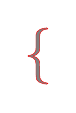
\begin{tikzpicture}[y=1cm, x=1cm, yscale=\globalscale,xscale=\globalscale, every node/.append style={scale=\globalscale}, inner sep=0pt, outer sep=0pt]
\path [draw=red, fill=gray, scale=2, line width=.15pt] (11.2977, -6.3235).. controls (11.2977, -6.059) and (11.139, -6.059) .. (10.8744, -6.0325).. controls (8.7842, -5.9002) and (7.8052, -4.7096) .. (7.5671, -3.7571).. controls (7.4877, -3.466) and (7.4877, -3.4131) .. (7.4877, -2.4871) -- (7.4877, 1.4817).. controls (7.4877, 2.2754) and (7.4877, 3.6248) .. (7.4348, 3.8894).. controls (7.0908, 5.6356) and (5.3975, 6.3235) .. (4.3656, 6.6146).. controls (7.4877, 7.5142) and (7.4877, 9.3927) .. (7.4877, 10.1335) -- (7.4877, 14.896).. controls (7.4877, 16.801) and (7.4877, 17.3831) .. (8.1227, 18.0446).. controls (8.599, 18.5208) and (9.2075, 19.1558) .. (11.0596, 19.2617).. controls (11.1919, 19.2881) and (11.2977, 19.394) .. (11.2977, 19.5527).. controls (11.2977, 19.8438) and (11.086, 19.8438) .. (10.7685, 19.8438).. controls (8.1227, 19.8438) and (5.7679, 18.4944) .. (5.715, 16.5894) -- (5.715, 11.7475).. controls (5.715, 9.2604) and (5.715, 8.8371) .. (5.0271, 8.0963).. controls (4.6567, 7.7258) and (3.9423, 7.0115) .. (2.2754, 6.9056).. controls (2.0902, 6.9056) and (1.905, 6.8792) .. (1.905, 6.6146).. controls (1.905, 6.35) and (2.0638, 6.35) .. (2.3283, 6.3235).. controls (3.466, 6.2442) and (5.715, 5.6885) .. (5.715, 3.0427) -- (5.715, -2.196).. controls (5.715, -3.7306) and (5.715, -4.6302) .. (7.0908, -5.6092).. controls (8.2285, -6.4029) and (9.9483, -6.6146) .. (10.7685, -6.6146).. controls (11.086, -6.6146) and (11.2977, -6.6146) .. (11.2977, -6.3235) -- cycle;
\end{tikzpicture}XXX

% 6. '%' percent symbol
XXX%

\begin{tikzpicture}[y=1cm, x=1cm, yscale=\globalscale,xscale=\globalscale, every node/.append style={scale=\globalscale}, inner sep=0pt, outer sep=0pt]
\path [draw=red, fill=gray, scale=2, line width=.15pt] (18.3356, 19.3146).. controls (18.3356, 19.6056) and (18.0975, 19.8438) .. (17.8065, 19.8438).. controls (17.5419, 19.8438) and (17.4096, 19.6585) .. (17.2508, 19.4733).. controls (15.9279, 17.6742) and (14.1552, 16.9598) .. (12.2238, 16.9598).. controls (10.3717, 16.9598) and (8.7313, 17.6212) .. (7.276, 18.9971).. controls (6.7733, 19.4469) and (6.2177, 19.8438) .. (5.371, 19.8438).. controls (3.3602, 19.8438) and (1.4817, 17.6212) .. (1.4817, 14.5256).. controls (1.4817, 11.3242) and (3.3867, 9.181) .. (5.371, 9.181).. controls (7.3025, 9.181) and (8.8106, 11.5358) .. (8.8106, 14.4992).. controls (8.8106, 14.8696) and (8.8106, 16.1131) .. (8.255, 17.489).. controls (9.9748, 16.51) and (11.2977, 16.3777) .. (12.2502, 16.3777).. controls (14.261, 16.3777) and (15.6104, 17.1979) .. (15.7692, 17.3038) -- (15.7956, 17.2773) -- (3.9158, -0.4233).. controls (3.6777, -0.7673) and (3.6777, -0.9525) .. (3.6777, -0.9525).. controls (3.6777, -1.2435) and (3.9423, -1.4817) .. (4.2069, -1.4817).. controls (4.4715, -1.4817) and (4.5244, -1.3758) .. (4.736, -1.0848) -- (18.124, 18.8383).. controls (18.2827, 19.0765) and (18.3356, 19.1558) .. (18.3356, 19.3146) -- cycle(20.5317, 3.8365).. controls (20.5317, 6.8792) and (18.9706, 9.181) .. (17.0921, 9.181).. controls (15.0813, 9.181) and (13.2027, 6.9585) .. (13.2027, 3.8629).. controls (13.2027, 0.6615) and (15.1077, -1.4817) .. (17.0921, -1.4817).. controls (19.0235, -1.4817) and (20.5317, 0.8731) .. (20.5317, 3.8365) -- cycle(8.1492, 14.5256).. controls (8.1492, 11.6681) and (6.7733, 9.7631) .. (5.3975, 9.7631).. controls (4.8683, 9.7631) and (3.1221, 10.1071) .. (3.1221, 14.4992).. controls (3.1221, 18.9177) and (4.8419, 19.2617) .. (5.3975, 19.2617).. controls (6.7998, 19.2617) and (8.1492, 17.3038) .. (8.1492, 14.5256) -- cycle(19.8702, 3.8629).. controls (19.8702, 1.0054) and (18.4944, -0.8996) .. (17.1185, -0.8996).. controls (16.5894, -0.8996) and (14.8431, -0.5556) .. (14.8431, 3.8365).. controls (14.8431, 8.255) and (16.5629, 8.599) .. (17.1185, 8.599).. controls (18.5208, 8.599) and (19.8702, 6.641) .. (19.8702, 3.8629) -- cycle;
\end{tikzpicture}XXX



%%%%%     TEST for 'lmm' other symbols      %%%%%
\section{lmm other symbols}
% 1. '{' symbol
XXX%
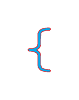
\begin{tikzpicture}[y=1cm, x=1cm, yscale=\globalscale,xscale=\globalscale, every node/.append style={scale=\globalscale}, inner sep=0pt, outer sep=0pt]
\path [draw=red, fill=cyan, scale=2, line width=.15pt] (12.2767, -1.6933).. controls (12.2767, -1.2435) and (11.9327, -1.1642) .. (11.721, -1.1642).. controls (7.62, -1.0583) and (7.62, 0.1058) .. (7.62, 1.0319) -- (7.62, 5.4504).. controls (7.62, 6.059) and (7.5406, 7.0908) .. (5.7415, 8.0698).. controls (7.1967, 8.9165) and (7.5935, 9.7367) .. (7.62, 10.3452).. controls (7.62, 10.3452) and (7.62, 15.8221) .. (7.7258, 16.0602).. controls (8.255, 17.1715) and (10.795, 17.3038) .. (11.8269, 17.3038).. controls (11.9327, 17.3038) and (12.2767, 17.436) .. (12.2767, 17.8594).. controls (12.2767, 18.4415) and (11.7475, 18.4415) .. (11.3771, 18.4415).. controls (9.5779, 18.4415) and (6.7469, 18.1769) .. (6.2971, 15.9015).. controls (6.2706, 15.7427) and (6.2706, 11.1919) .. (6.2706, 11.1919).. controls (6.2706, 10.0542) and (6.2442, 9.6044) .. (5.1329, 9.1017).. controls (4.101, 8.6783) and (2.6988, 8.6519) .. (2.0373, 8.6519).. controls (1.9315, 8.6519) and (1.5875, 8.5196) .. (1.5875, 8.0963).. controls (1.5875, 7.6465) and (1.8785, 7.5406) .. (2.1167, 7.5406).. controls (3.0427, 7.4877) and (6.2177, 7.276) .. (6.2706, 5.6621) -- (6.2706, 1.1113).. controls (6.2706, 0.3704) and (6.2706, -0.7673) .. (7.5671, -1.4817).. controls (8.6783, -2.0902) and (10.1335, -2.2754) .. (11.3771, -2.2754).. controls (11.7475, -2.2754) and (12.2767, -2.2754) .. (12.2767, -1.6933) -- cycle;
\end{tikzpicture}XXX

% 2. '$' symbol
XXX%

\begin{tikzpicture}[y=1cm, x=1cm, yscale=\globalscale,xscale=\globalscale, every node/.append style={scale=\globalscale}, inner sep=0pt, outer sep=0pt]
\path [draw=red, fill=blue, scale=2, line width=.15pt] (12.2502, 4.3921).. controls (12.2502, 5.6621) and (11.4829, 8.2285) .. (7.5142, 8.9694) -- (7.5142, 15.1871).. controls (8.7842, 15.0283) and (10.2658, 14.605) .. (10.795, 12.8852).. controls (10.451, 12.6206) and (10.3452, 12.356) .. (10.3452, 12.0915).. controls (10.3452, 11.6152) and (10.7156, 11.1654) .. (11.2713, 11.1654).. controls (11.721, 11.1654) and (12.2502, 11.43) .. (12.2502, 12.2238).. controls (12.2502, 14.2081) and (10.795, 16.0338) .. (7.5142, 16.3248) -- (7.5142, 17.5948).. controls (7.5142, 17.9123) and (7.5142, 18.4415) .. (6.9585, 18.4415).. controls (6.3765, 18.4415) and (6.3765, 17.9123) .. (6.3765, 17.5948) -- (6.3765, 16.2983).. controls (3.3073, 15.9544) and (1.614, 13.9965) .. (1.614, 12.0915).. controls (1.614, 11.4565) and (1.7992, 8.7048) .. (6.3765, 7.8581) -- (6.3765, 0.979).. controls (4.736, 1.1906) and (3.519, 1.8521) .. (3.0163, 3.5719).. controls (3.3338, 3.7571) and (3.519, 3.9158) .. (3.519, 4.3921).. controls (3.519, 5.0006) and (3.0163, 5.371) .. (2.5929, 5.371).. controls (2.3813, 5.371) and (1.614, 5.2652) .. (1.614, 4.2598).. controls (1.614, 2.1167) and (3.1485, 0.1588) .. (6.3765, -0.1588) -- (6.3765, -1.4288).. controls (6.3765, -1.7463) and (6.3765, -2.2754) .. (6.9585, -2.2754).. controls (7.5142, -2.2754) and (7.5142, -1.7463) .. (7.5142, -1.4288) -- (7.5142, -0.1588).. controls (10.9008, 0.3704) and (12.2502, 2.5929) .. (12.2502, 4.3921) -- cycle(6.3765, 9.2075).. controls (4.3656, 9.5779) and (2.831, 10.6892) .. (2.831, 12.1973).. controls (2.831, 13.626) and (4.2333, 14.8431) .. (6.3765, 15.2135) -- cycle(11.0331, 4.2863).. controls (11.0331, 2.7781) and (9.7102, 1.3758) .. (7.5142, 0.979) -- (7.5142, 7.62).. controls (9.7896, 7.1702) and (11.0331, 5.7944) .. (11.0331, 4.2863) -- cycle;
\end{tikzpicture}XXX

% 6. '%' percent symbol
XXX%

\begin{tikzpicture}[y=1cm, x=1cm, yscale=\globalscale,xscale=\globalscale, every node/.append style={scale=\globalscale}, inner sep=0pt, outer sep=0pt]
\path [draw=red, fill=gray, scale=2, line width=.15pt] (5.2123, 15.0548).. controls (5.2123, 16.9863) and (4.3127, 18.4415) .. (3.0956, 18.4415).. controls (1.8785, 18.4415) and (1.0054, 16.9333) .. (1.0054, 15.0813).. controls (1.0054, 13.1233) and (1.905, 11.6681) .. (3.0956, 11.6681).. controls (4.3392, 11.6681) and (5.2123, 13.1763) .. (5.2123, 15.0548) -- cycle(11.4565, 17.7535).. controls (11.4565, 18.0975) and (11.139, 18.4415) .. (10.7685, 18.4415).. controls (10.3188, 18.4415) and (10.1335, 18.0181) .. (10.0277, 17.7535) -- (2.5665, -1.0848).. controls (2.4606, -1.3229) and (2.4077, -1.4552) .. (2.4077, -1.5875).. controls (2.4077, -1.9579) and (2.7252, -2.2754) .. (3.0956, -2.2754).. controls (3.466, -2.2754) and (3.6248, -2.0373) .. (3.7306, -1.8256) -- (11.2977, 17.2508).. controls (11.4035, 17.489) and (11.4565, 17.6212) .. (11.4565, 17.7535) -- cycle(12.8588, 1.0848).. controls (12.8588, 2.9369) and (12.0121, 4.4715) .. (10.7685, 4.4715).. controls (9.525, 4.4715) and (8.6519, 2.9369) .. (8.6519, 1.0848).. controls (8.6519, -0.7673) and (9.525, -2.2754) .. (10.7685, -2.2754).. controls (12.0121, -2.2754) and (12.8588, -0.7673) .. (12.8588, 1.0848) -- cycle(4.2333, 15.0813).. controls (4.2333, 13.6525) and (3.4925, 12.8323) .. (3.0956, 12.8323).. controls (2.7252, 12.8323) and (1.9844, 13.6525) .. (1.9844, 15.0813).. controls (1.9844, 16.3777) and (2.6723, 17.2773) .. (3.0956, 17.2773).. controls (3.519, 17.2773) and (4.2333, 16.3777) .. (4.2333, 15.0813) -- cycle(11.8798, 1.0848).. controls (11.8798, -0.3175) and (11.139, -1.1113) .. (10.7685, -1.1113).. controls (10.3717, -1.1113) and (9.6308, -0.3175) .. (9.6308, 1.0848).. controls (9.6308, 2.5135) and (10.3717, 3.3073) .. (10.7685, 3.3073).. controls (11.139, 3.3073) and (11.8798, 2.5135) .. (11.8798, 1.0848) -- cycle;
\end{tikzpicture}XXX
\end{document}